\section{Results}

In this section, we present the results obtained from our experiments and the performance benchmark, which was the time needed to generate a frame for live-view and the time it took for an image in the high-resolution mode to be processed and sent to the user. We also present qualitative results of the implemented style transferring network and a general overview of the final prototype's functioning.

\subsection{Pre-processing: face and emotion detection}


\begin{figure}[h]
    \centering
    \begin{subfigure}[t]{0.32\textwidth}
        \centering
        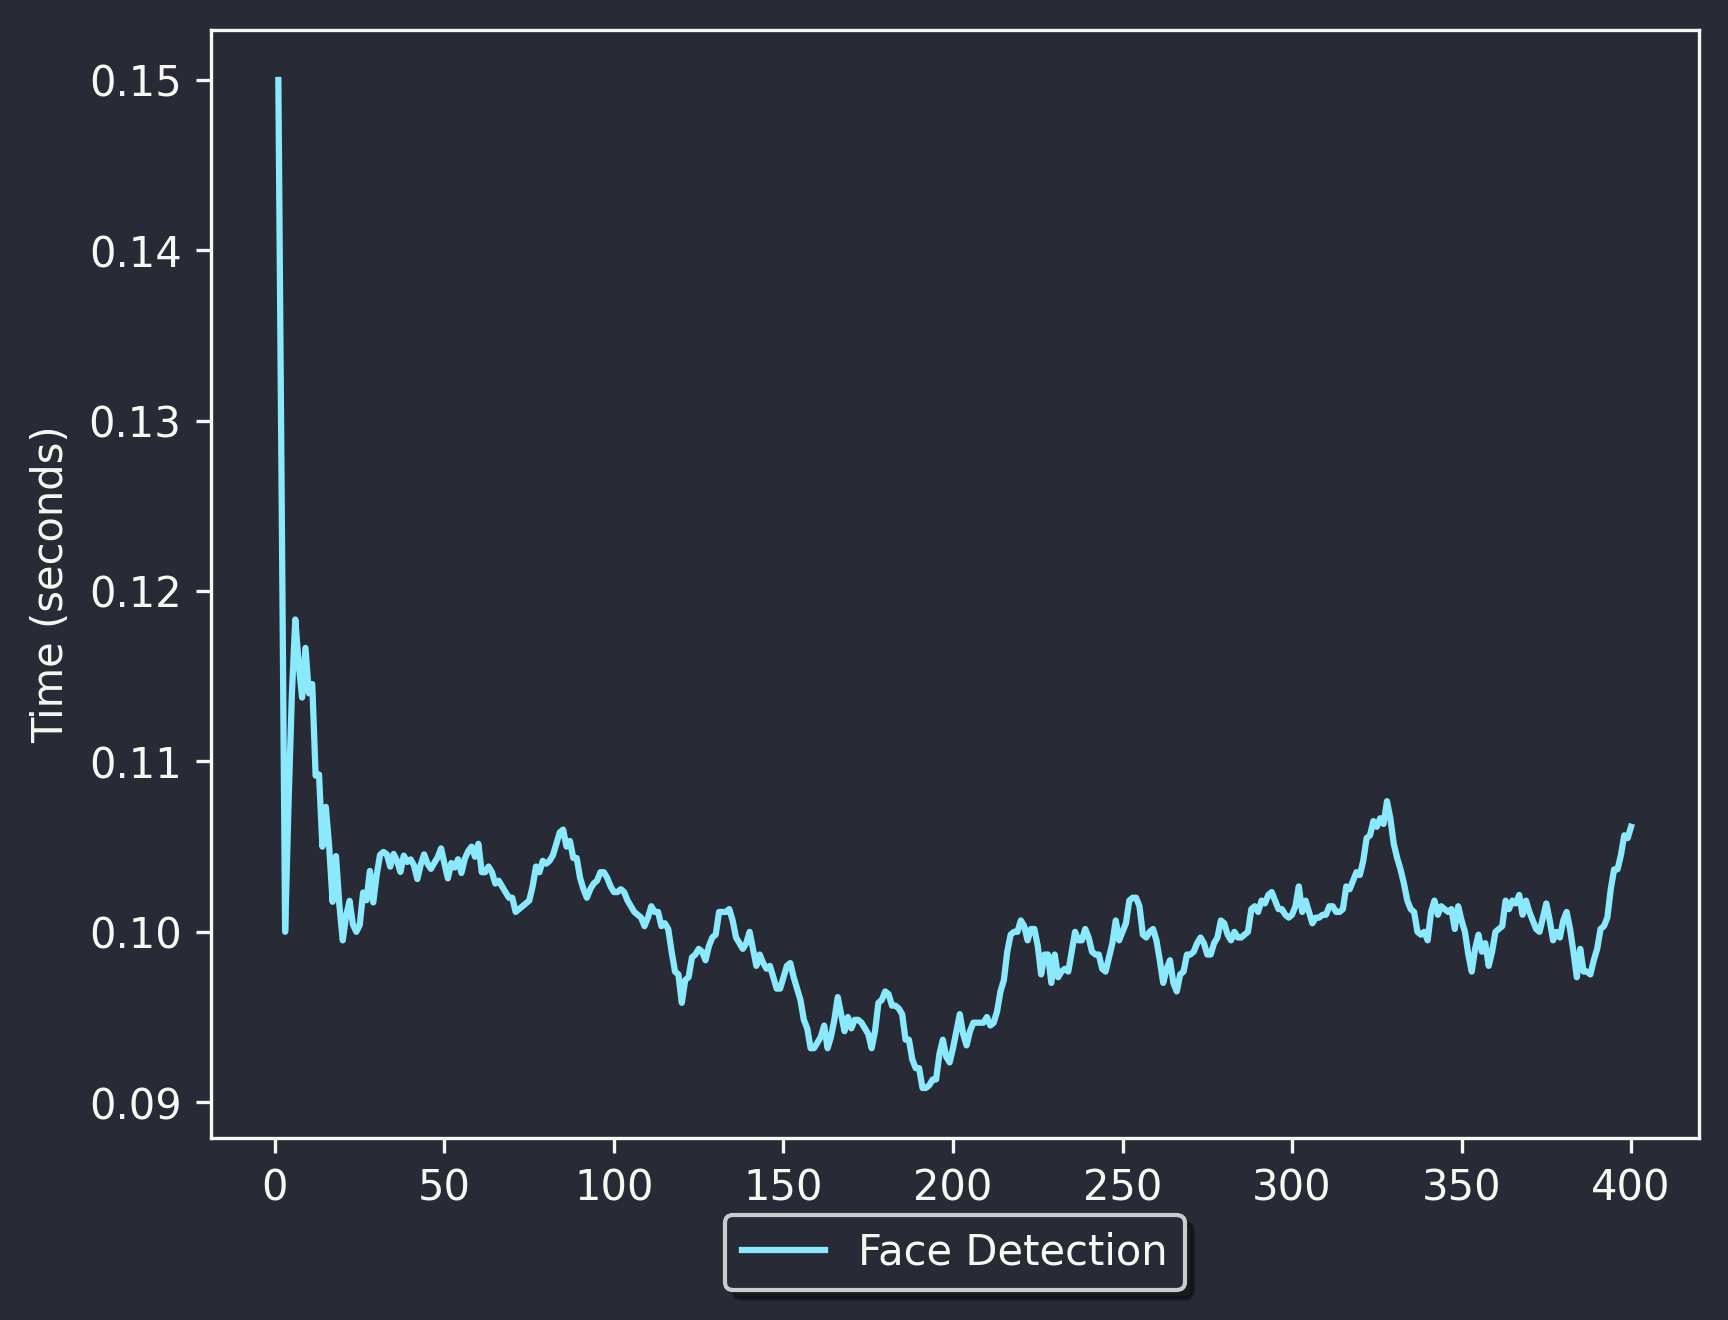
\includegraphics[width = \textwidth]{resources/faceFPS.png}
        \caption{Face detection time per frame.}\label{fig:faceFPS}
    \end{subfigure}
    \begin{subfigure}[t]{0.32\textwidth}
        \centering
        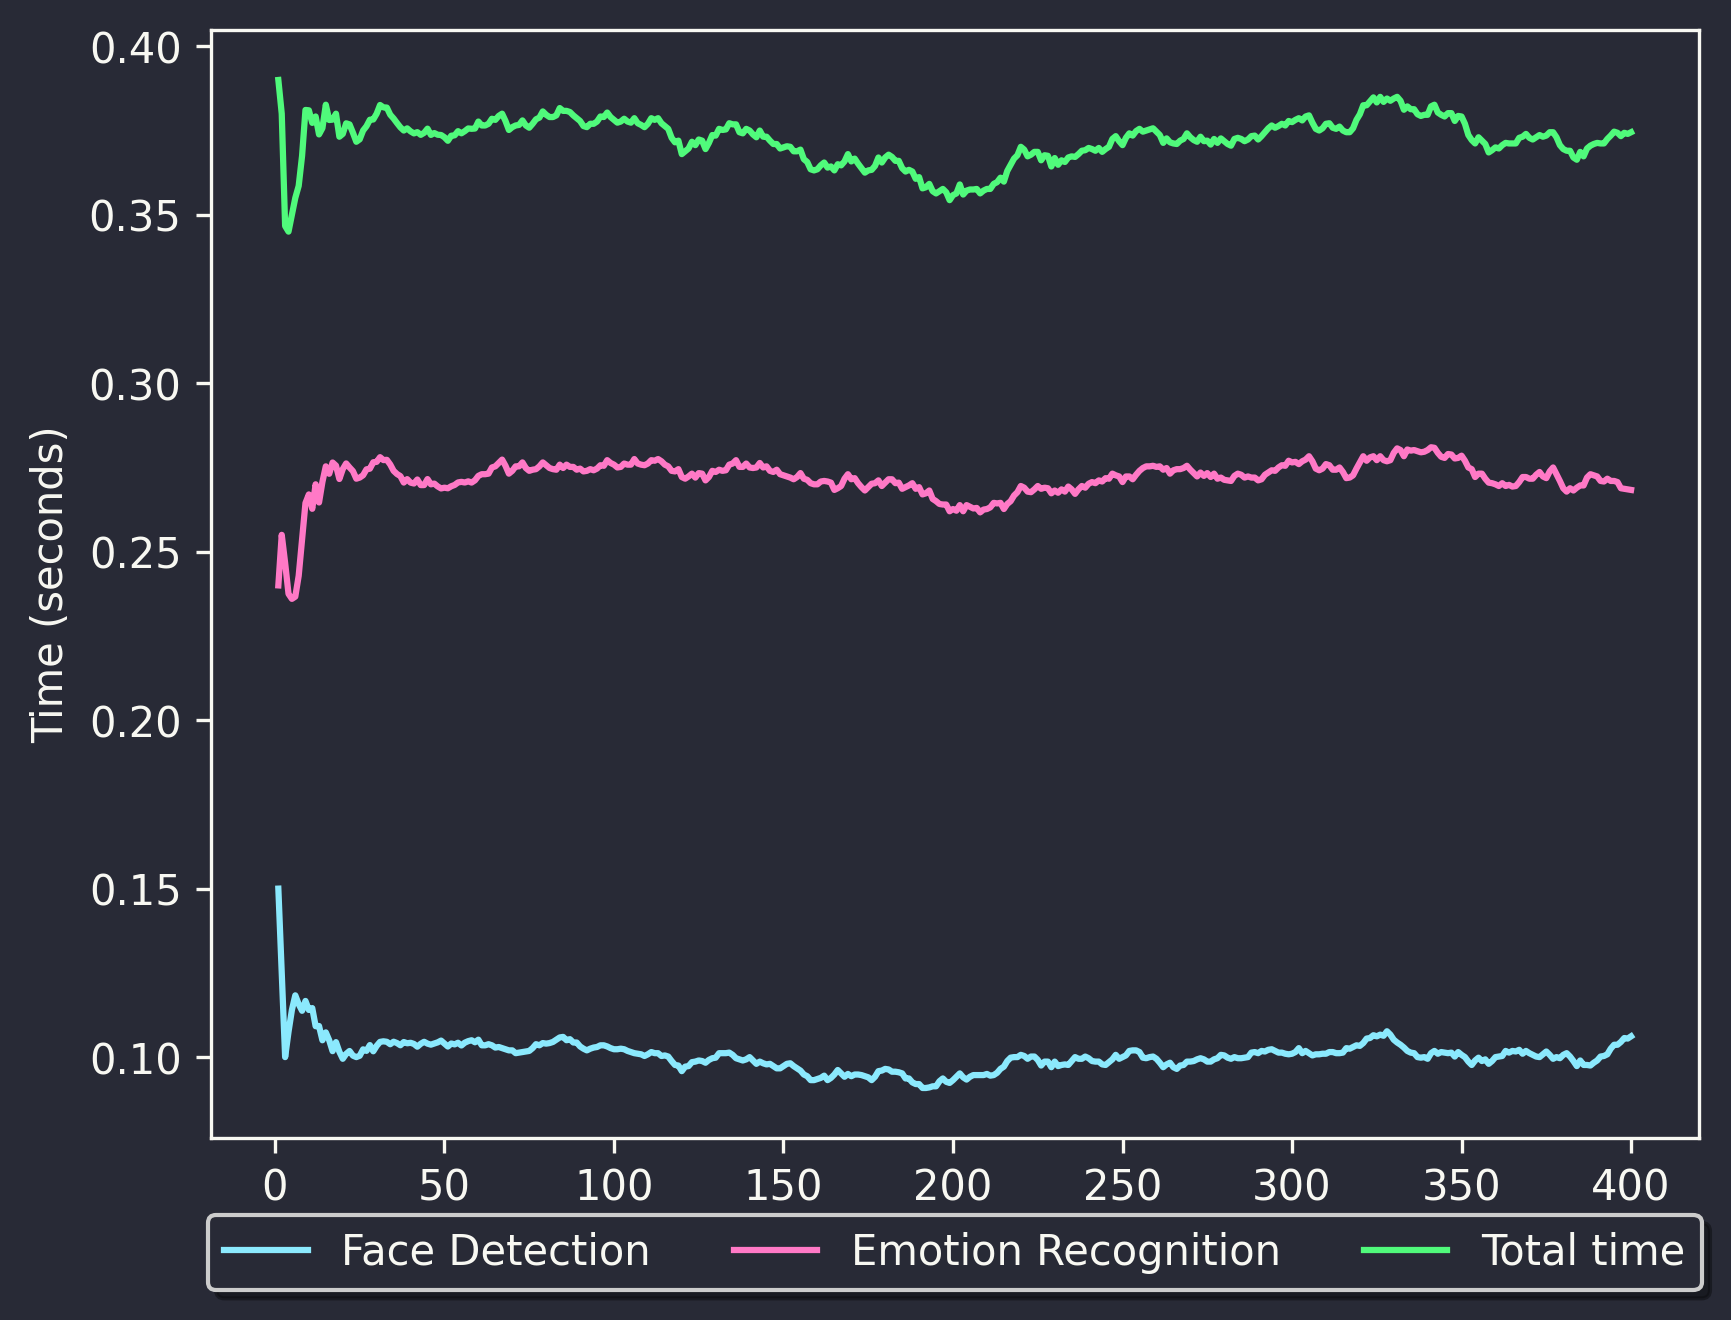
\includegraphics[width = \textwidth]{resources/face_emoFPS.png}
        \caption{Face, emotion detection and total time per frame.}\label{fig:faceemoFPS}
    \end{subfigure}
    \begin{subfigure}[t]{0.32\textwidth}
        \centering
        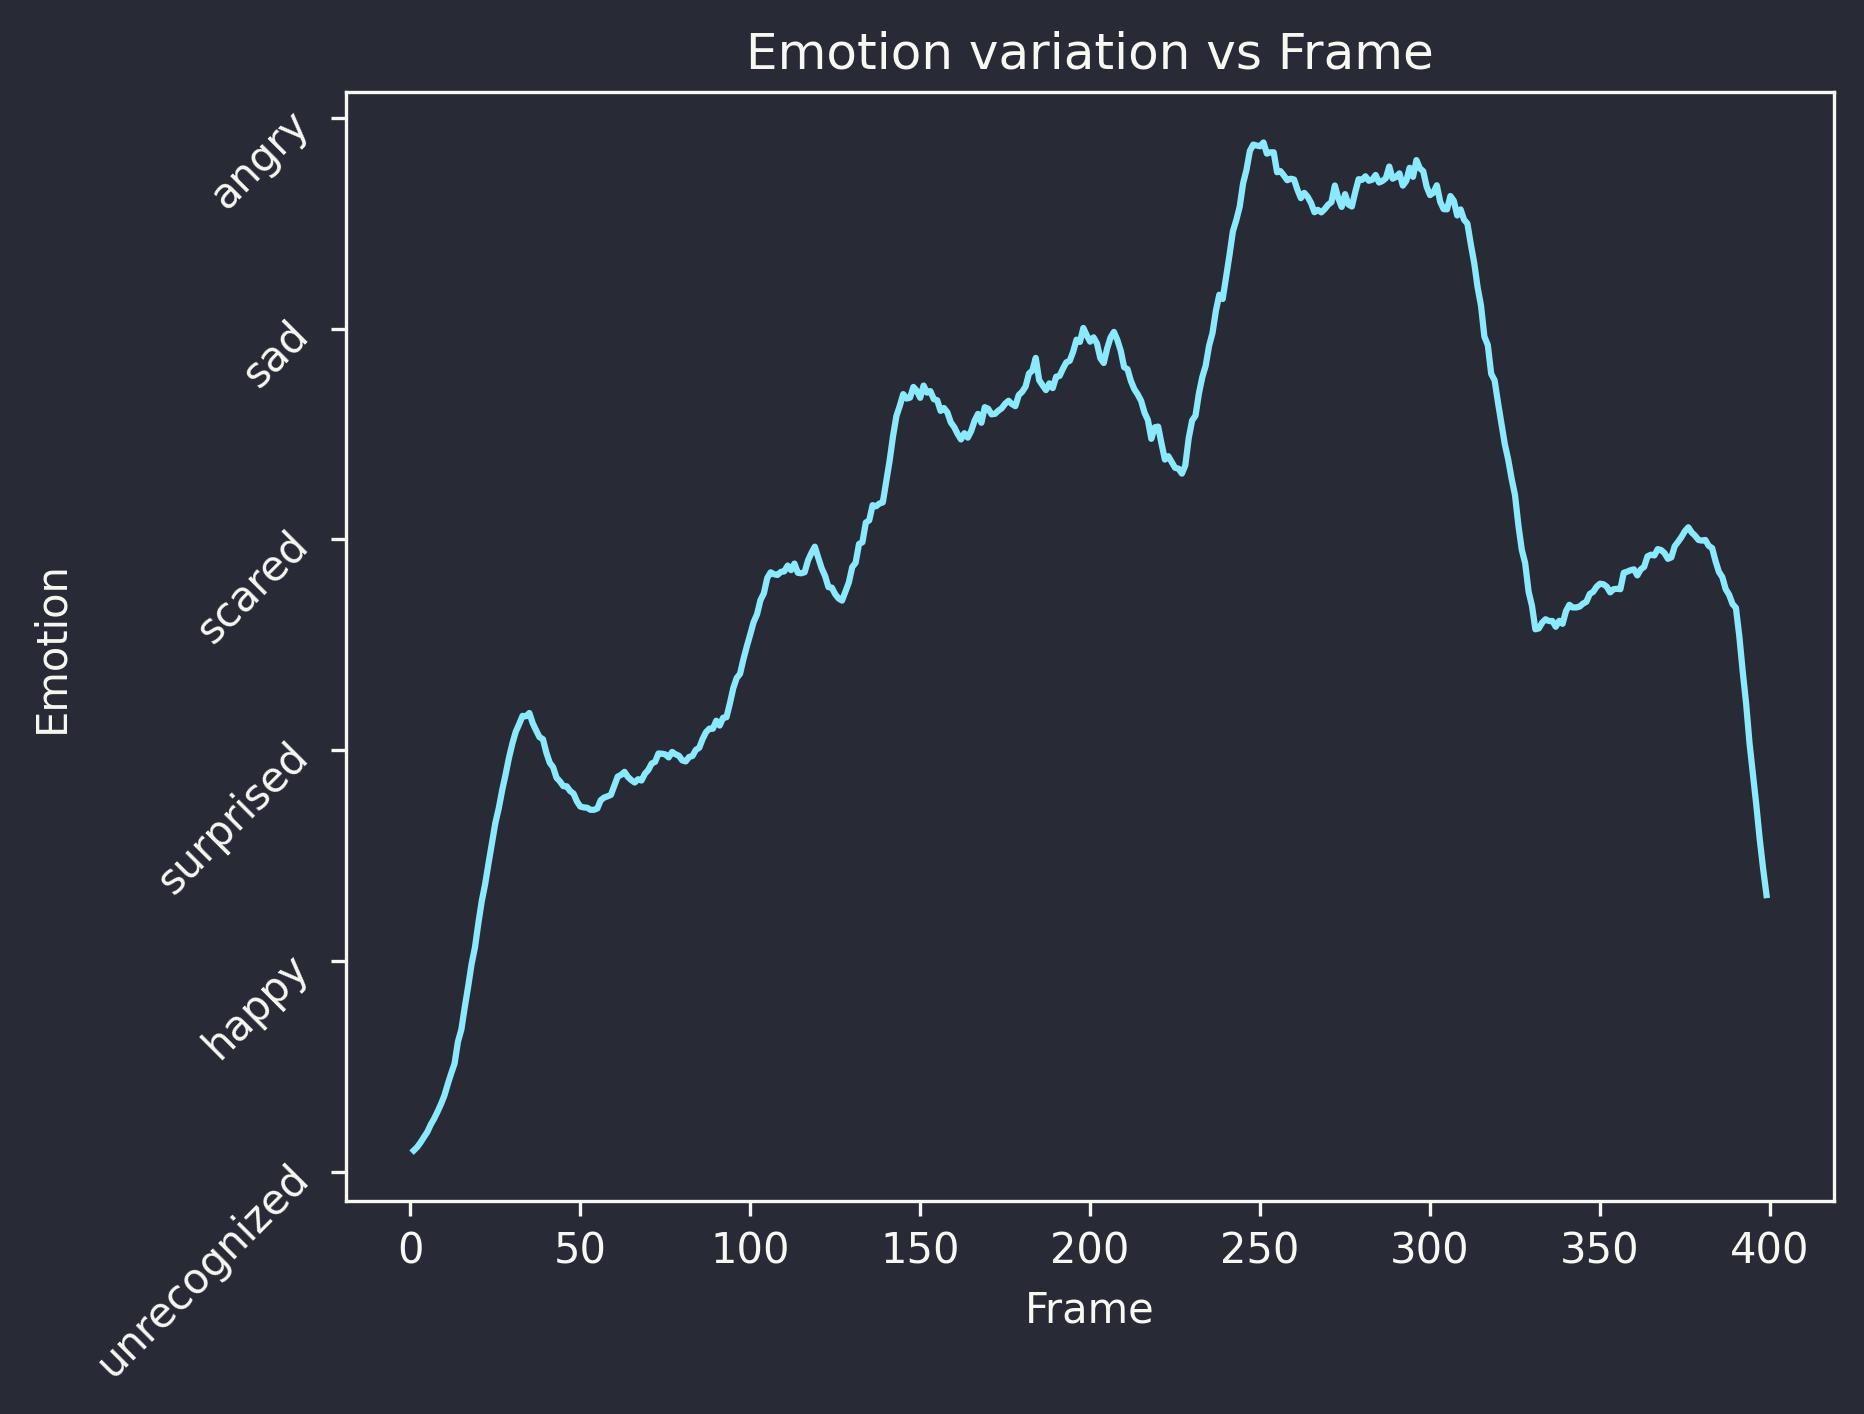
\includegraphics[width = \textwidth]{resources/emotionvsframe.png}
        \caption{Emotion variation by frame of a sample.}\label{fig:emotionvsframe}
    \end{subfigure}
    \caption{Performance of face and emotion recognition.}\label{fig:face_emo_bigtable}
\end{figure}



Our final implementation of face detection can produce results at an average of 0.1 seconds per frame on the Raspberry Pi's hardware, as seen in Figure \ref{fig:faceFPS}.


Our overall performance almost matches the original "sequential fully-CNN" model's performance at 65\% accuracy, but our implementation can complete the recognition of a cropped face's emotion in 0.28 seconds on average, as seen in figure \ref{fig:faceemoFPS}. We also captured a sample for the detected emotion variation for the same sample as our benchmarking run, as seen in figure \ref{fig:emotionvsframe}.


\begin{figure}[h]
    \centering
    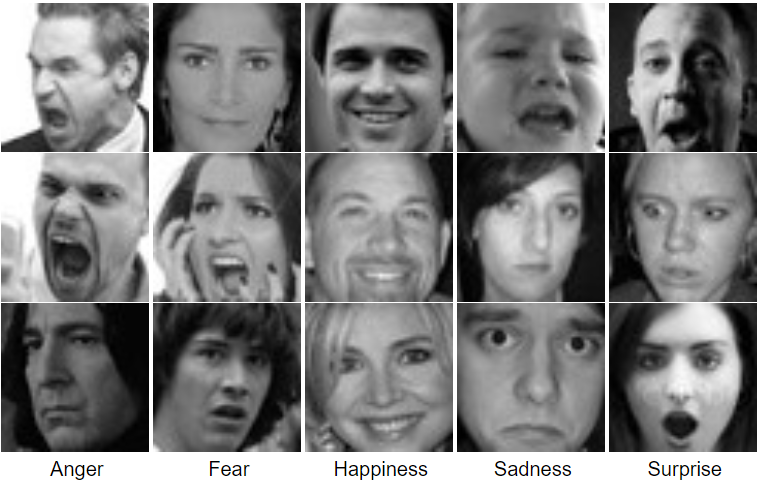
\includegraphics[width = 0.4\textwidth]{resources/emotion_faces_0.png}
    \caption{Emotion detection results sample.}\label{fig:emotion_faces}
\end{figure}



In figure \ref{fig:emotion_faces} you can see a small sample of the performance of our emotion recognition on the FER dataset, and on Table \ref{tab:acc_per_emotion} you can see the performance of the emotion recognition per emotion.

\begin{table}[h]
    \centering
    \begin{tabular}{ll}
        \hline
        \textbf{Emotion}   & \textbf{Accuracy} \\ \hline
        \textbf{Anger}     & 68\%              \\
        \textbf{Sadness}   & 67\%              \\
        \textbf{Fear}      & 60\%              \\
        \textbf{Surprise}  & 64\%              \\
        \textbf{Happiness} & 68\%              \\ \hline
    \end{tabular}
    \caption{Accuracy per emotion}
    \label{tab:acc_per_emotion}
\end{table}

We produced these results by running the network through a subset of images reserved for testing.

\subsection{Style transfer}


As discussed in the experiments section, we implemented StylePi using batch normalization instead of instance normalization. For the most part, this does not affect the quality of the images, but it does ocassionally generate interesting artifacts that produce a clearly different visual result as an effect of batch normalization, as seen in an example on Figure \ref{fig:style_norm_comp}. We believe that this difference, or "pattern-ization" of the image is the product of how batch normalization works, as we can see in the same figure how the "swirling" pattern of Van Gogh's starry night repeats itself in a regular manner. It is not clear to the author under what conditions this happens, as all models have exhibited this behaviour at some point of the experimental phase.


\begin{figure}[h]
    \centering
    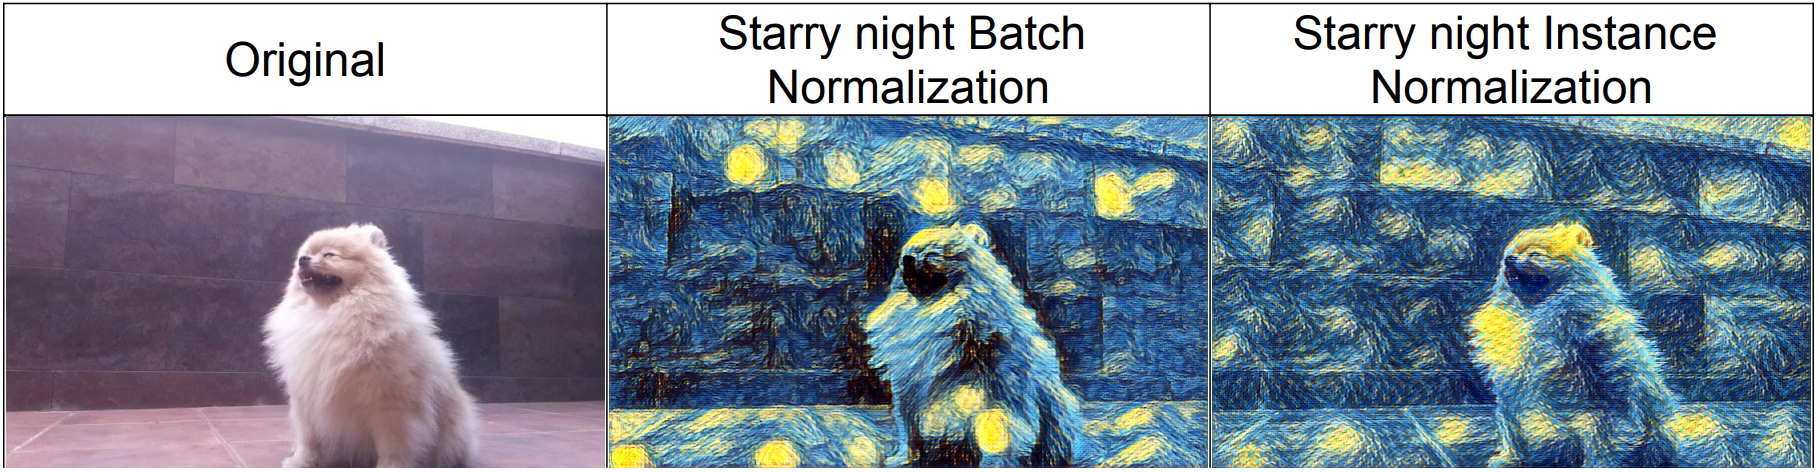
\includegraphics[width = 0.9\textwidth]{resources/style_norm_comp.png}
    \caption{Comparison of instance vs batch normalization}
    \label{fig:style_norm_comp}
\end{figure}

Ultimately, however, batch normalization was able to provide an average processing time of 0.47 seconds per frame over a 400 frame sample, as seen in Figure \ref{fig:finalFPS}.

\begin{figure}[h]
    \centering
    \begin{subfigure}[t]{0.45\textwidth}
        \centering
        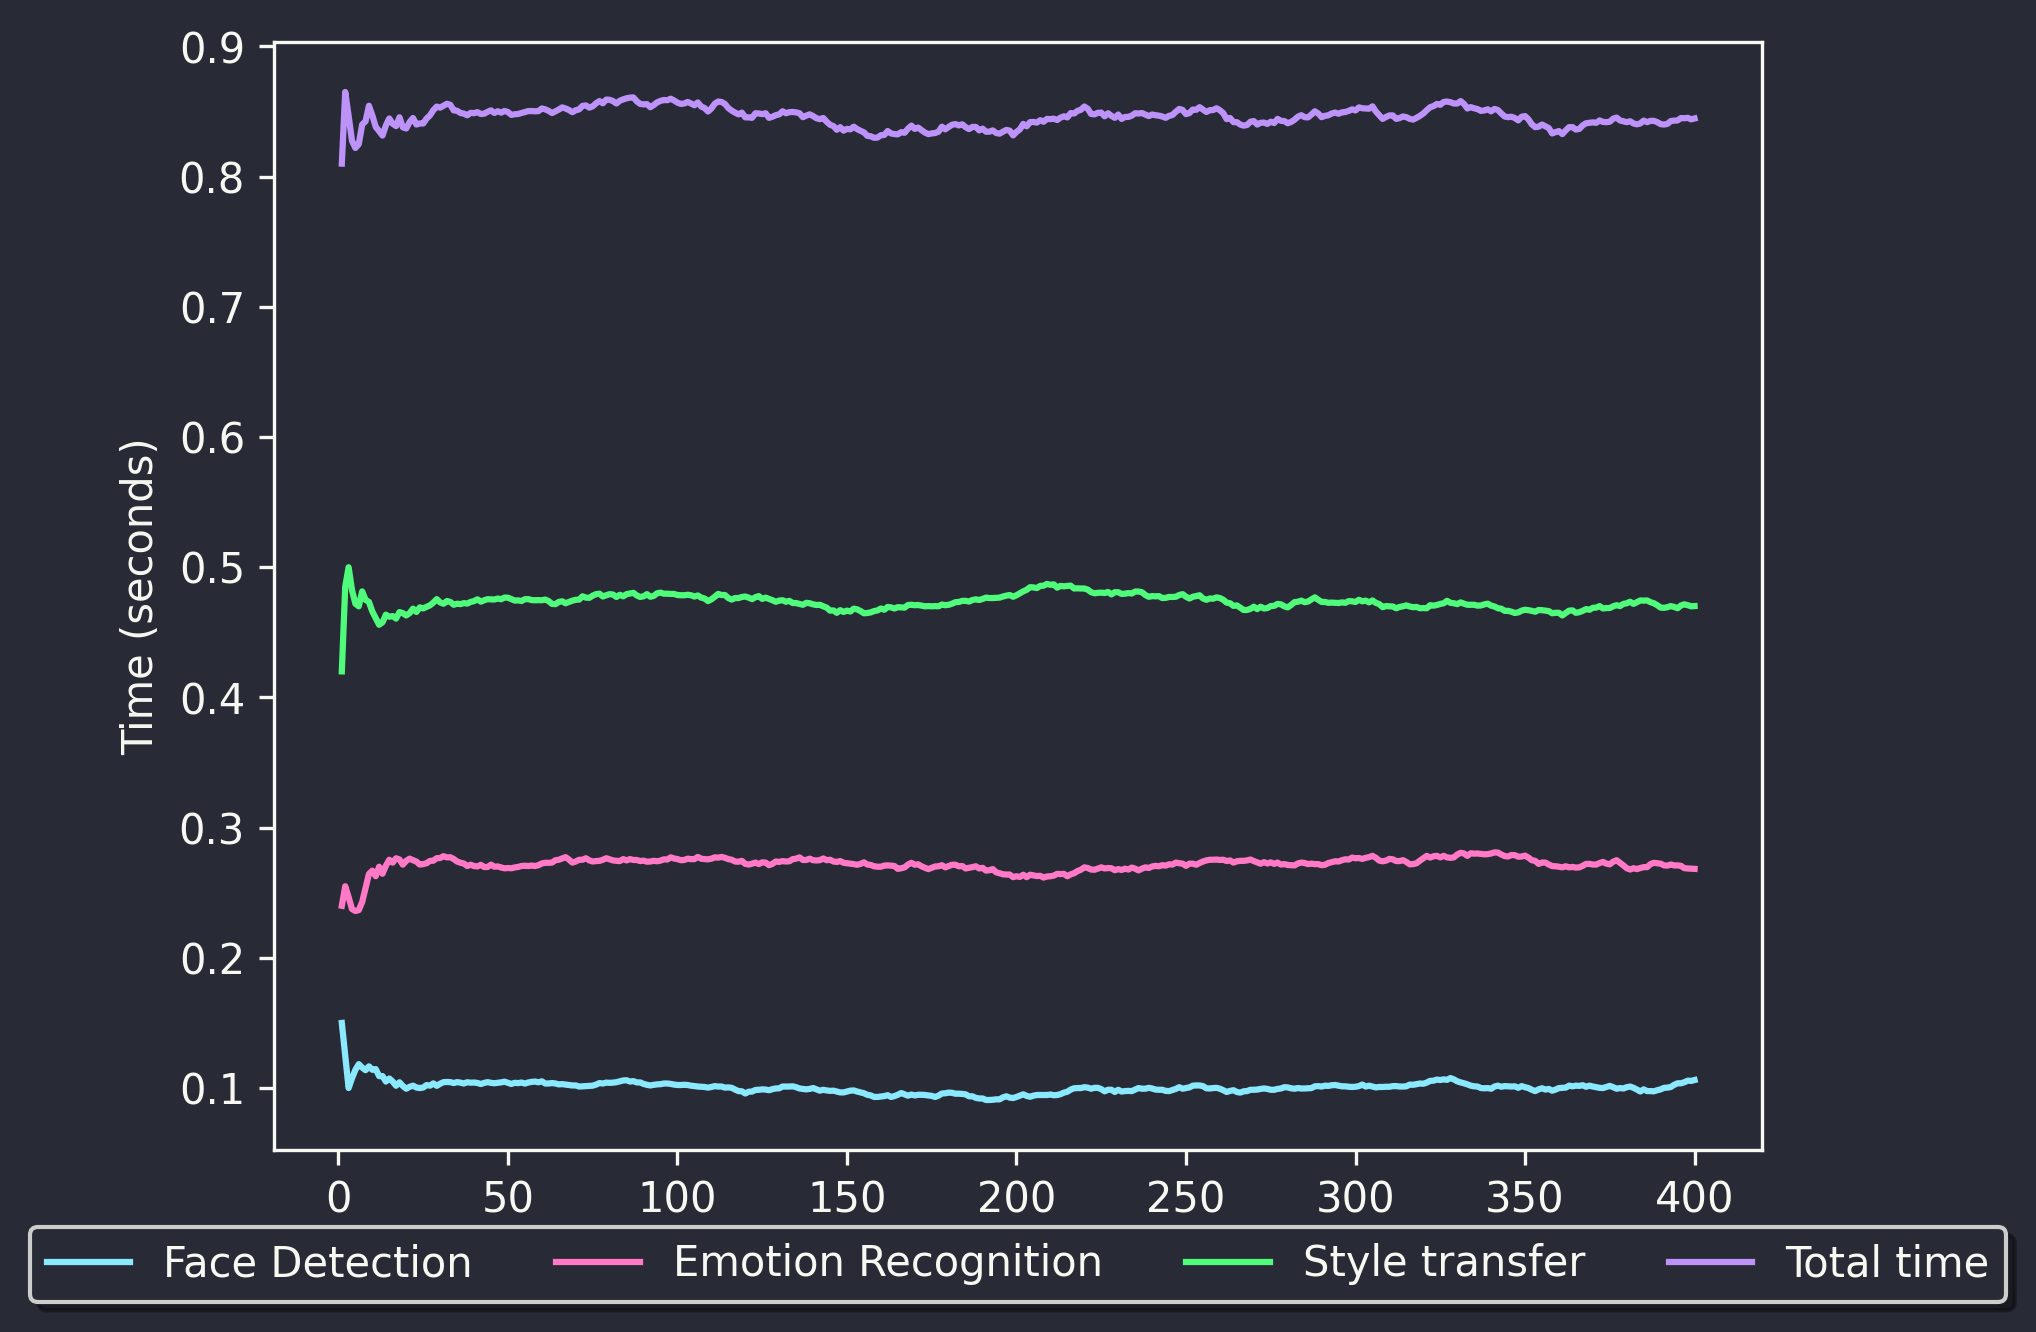
\includegraphics[height = 5.3cm]{resources/finalFPS.png}
        \caption{Performance of face/emotion detection and style transfer per frame.}\label{fig:finalFPS}
    \end{subfigure}
    \begin{subfigure}[t]{0.45\textwidth}
        \centering
        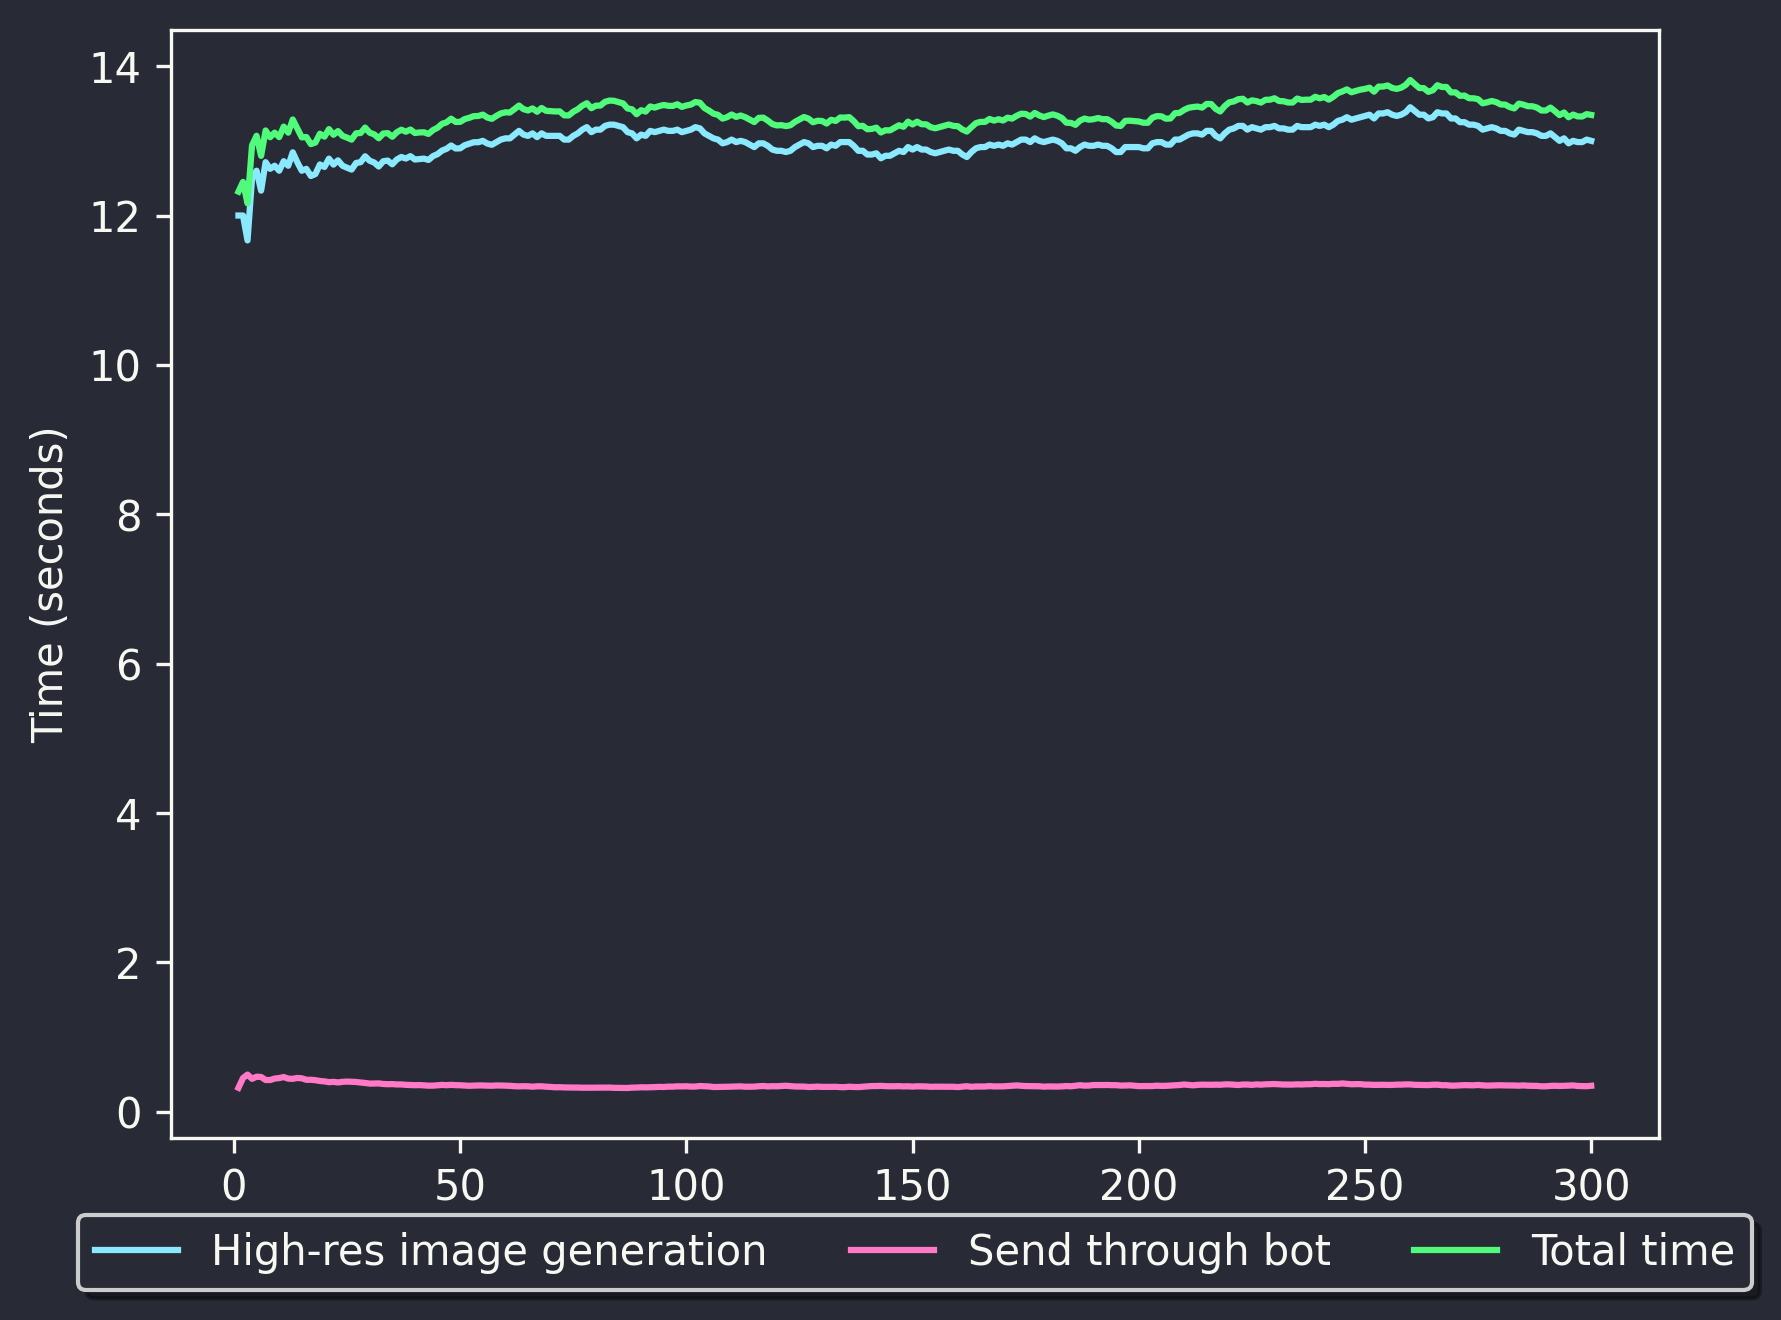
\includegraphics[height =5.3cm]{resources/result_generation_time.png}
        \caption{Total time needed to generate a high resolution image and send it through the bot.}
        \label{fig:result_generation_time}
    \end{subfigure}
    \caption{Final performance per frame and time needed to generate high-resolution images.}\label{fig:final_results_big_fig}
\end{figure}

\subsection{Final MVP performance}

In figure \ref{fig:style_results_grid} you can see the available styles and their associated emotions for a sample image. This figure also includes the output of both modes of the StylePi network: a high resolution and a low-resolution output.

\begin{figure}[h]
    \centering
    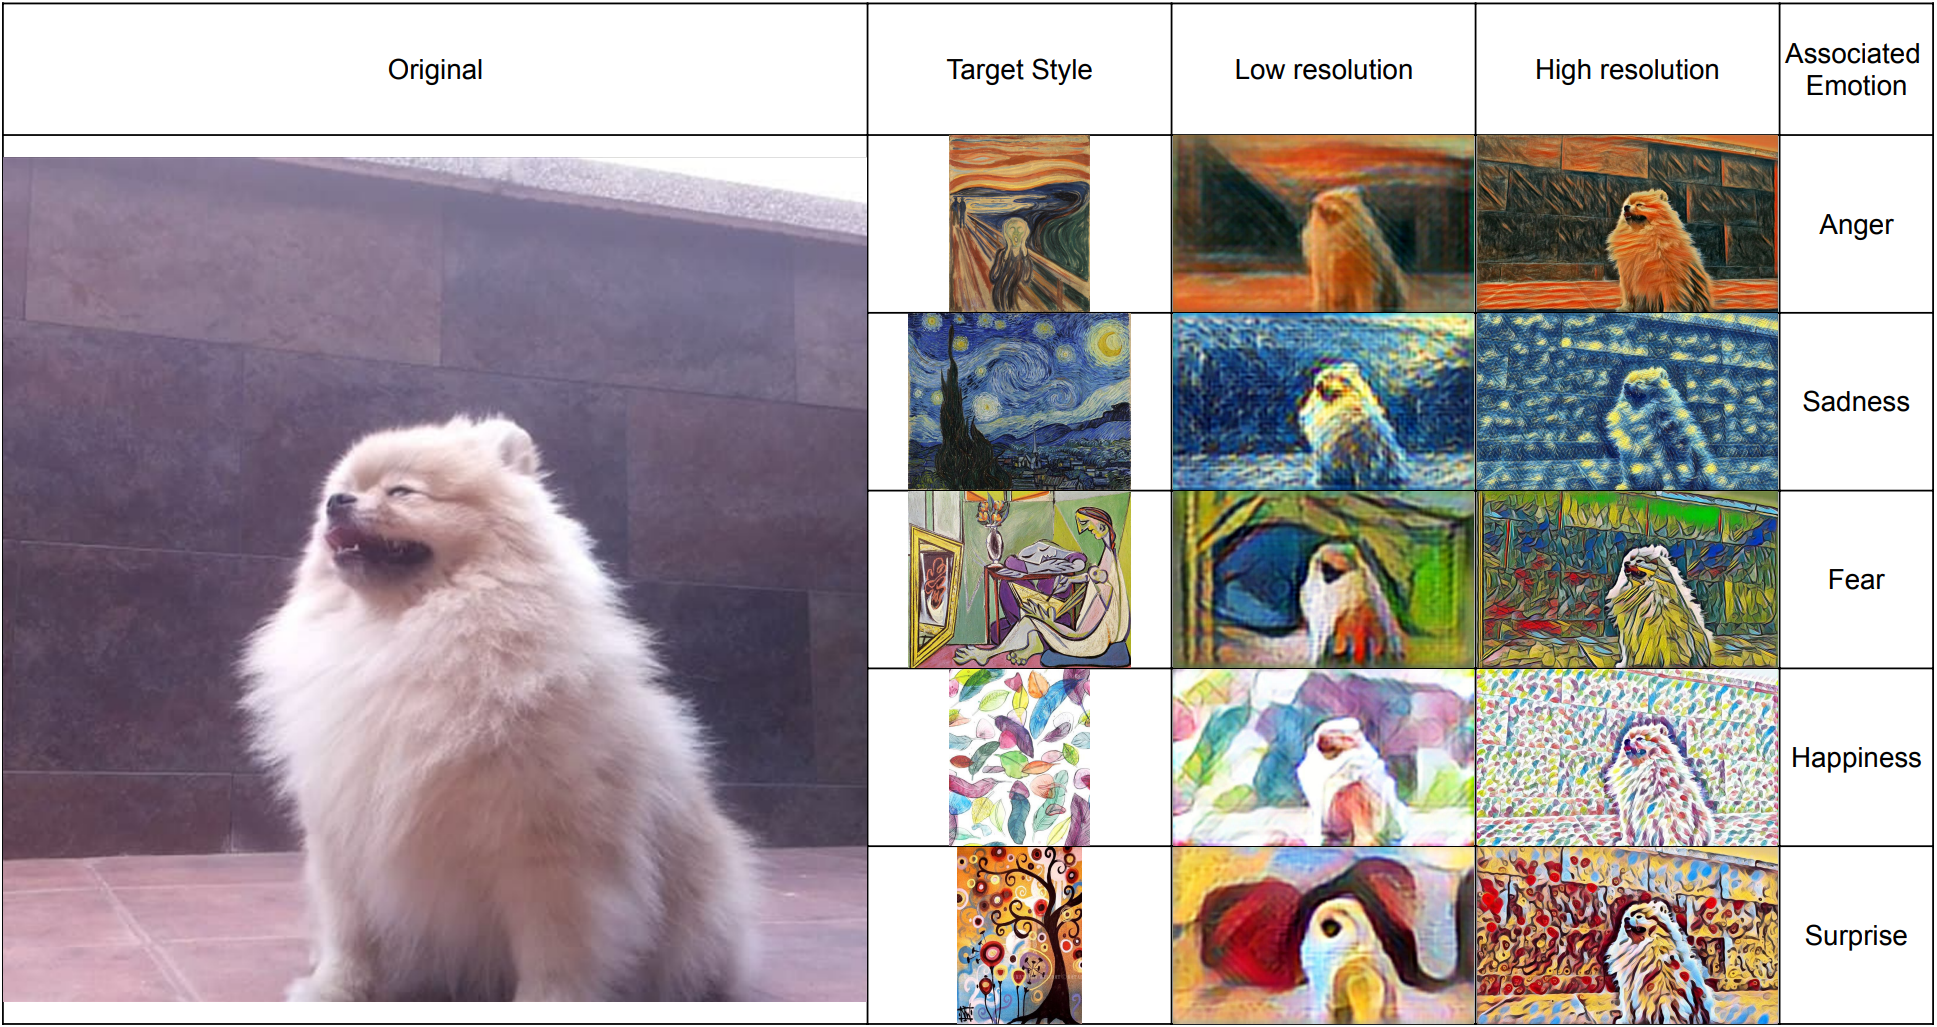
\includegraphics[width = \textwidth]{resources/styletransfer_emogrid.png}
    \caption{Available style transfers for emotion context switching sample. From top to bottom:
        \emph{The scream} By Edvard Munch,
        \emph{The Starry Night} By Vincent Van Gogh,
        \emph{La Musa (Mujer Leyendo)} By Pablo Picasso,
        \emph{Feathers} By Kathryn Corlett,
        \emph{June tree} By Natasha wescoat.
    } \label{fig:style_results_grid}
\end{figure}
The user can request all images generated by the MVP through the provided Telegram bot. The average time needed to generate a high-resolution style transfer of the camera's captured frame and send it through the telegram bot to the user can be seen in Figure \ref{fig:result_generation_time}. We found that selecting the minimum number of images (one) vs. selecting the maximum number of images (five: Original, Lowres, Lowres upscaled, Highres, Highres upscaled) did not impact the time it takes for the bot to send them.